%% Based on a TeXnicCenter-Template by Gyorgy SZEIDL.
%%%%%%%%%%%%%%%%%%%%%%%%%%%%%%%%%%%%%%%%%%%%%%%%%%%%%%%%%%%%%

%----------------------------------------------------------
%

\documentclass{beamer}%
%\makeatletter
\def\Hy@xspace@end{}
\makeatother
%\let\ifGm@compatii\relax\makeatother
%
%----------------------------------------------------------%

\usetheme{Warsaw}
\setbeamercovered{transparent}

\usepackage{ngerman}						%%Deutsche Sprachdatei
\usepackage[latin1]{inputenc}		%%Umlaute
%%%% --> latin1 bleibt da drin^^ bei utf8 gehts net
\usepackage[T1]{fontenc}				%%neue Kodierung

\usepackage{amsmath}%
\usepackage{amsfonts}%
\usepackage{amssymb}%
\usepackage{graphicx}
\usepackage{lscape}

\title[SEP 2011]{Simualtion von Achterbahnen}
\subtitle{SEP 2011}
\author{\tiny{Matthias Christian Daniel Simon  Robin Konstantin Marco}}
\institute[TU-BS]{Technische Universit"at Carolo-Wilhelmina zu Braunschweig}
\date{25.05.2011}


\begin{document}

	\begin{frame}
		\titlepage
	\end{frame}
	
	\section*{Inhalt}
	\begin{frame}{Inhalt}
		\tableofcontents
	\end{frame}
	
	\section{Zielsetzungen}
	\begin{frame}{Zielsetzungen}
	\begin{itemize}
	\item Ingenieursm"a"sige Konstruktion einer Achterbahn
		\begin{itemize}
			\item Physikalisch korrekte Wiedergabe
			\item Bodenfl"ache, 2 parallele Schienen, Quertr"ager
		\end{itemize}
		\item 2D-Visualierung der Beschleunigung
	\end{itemize}

	\end{frame}
	
	

	
	\subsection{Vor der Simulation}
	\begin{frame}{Visualierung}
		\begin{figure}
			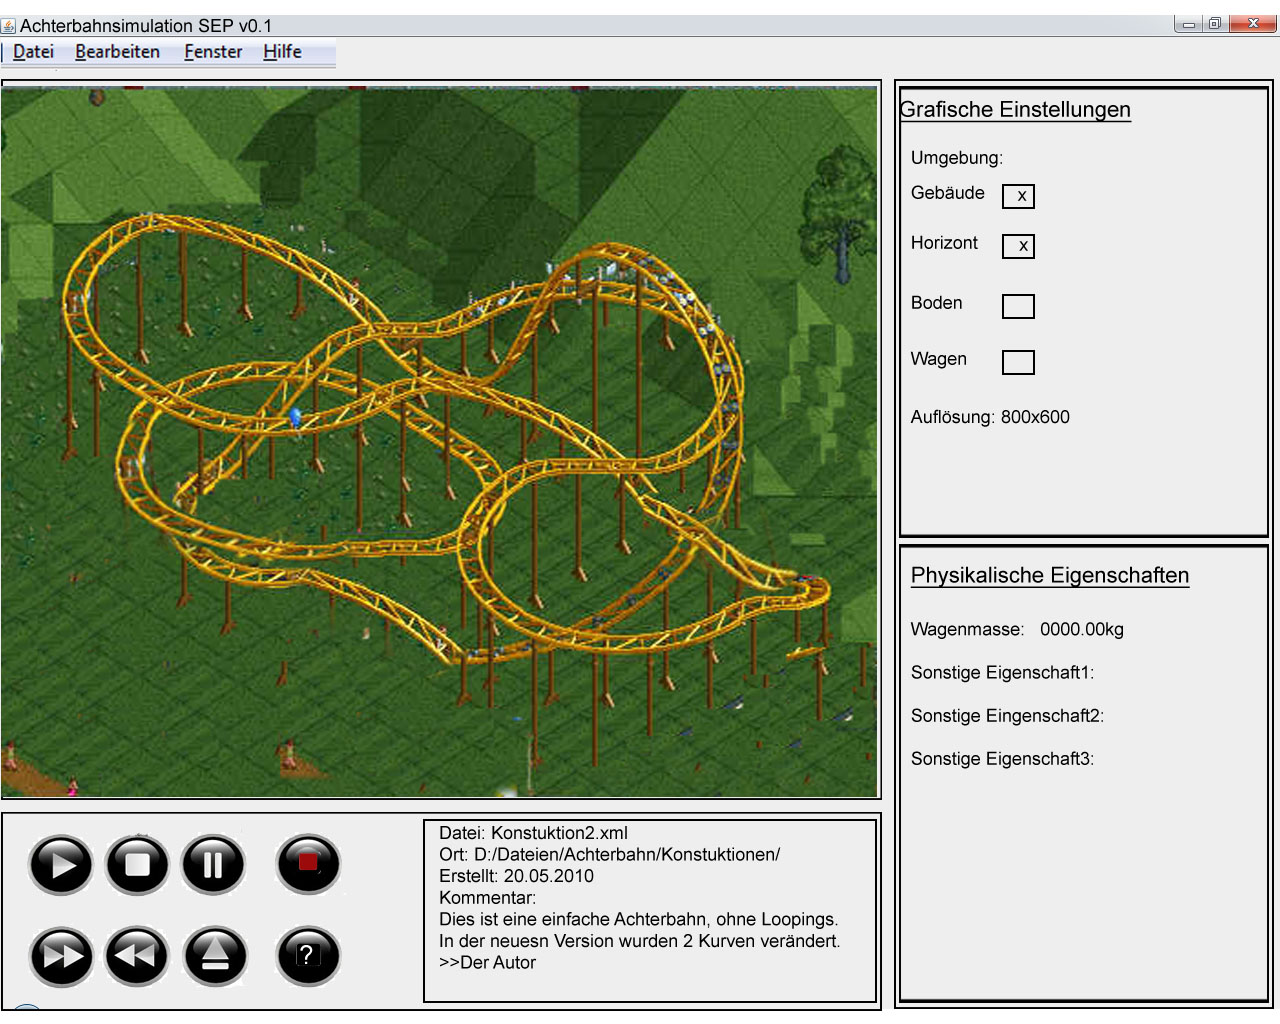
\includegraphics[width=0.75\linewidth]{GUI_v3.jpg}
			\caption{Vor dem Starten}
		\end{figure}
	\end{frame}
	
	\subsection{W"ahrend der Simulation}
		\begin{frame}{Visualierung}
		\begin{figure}
			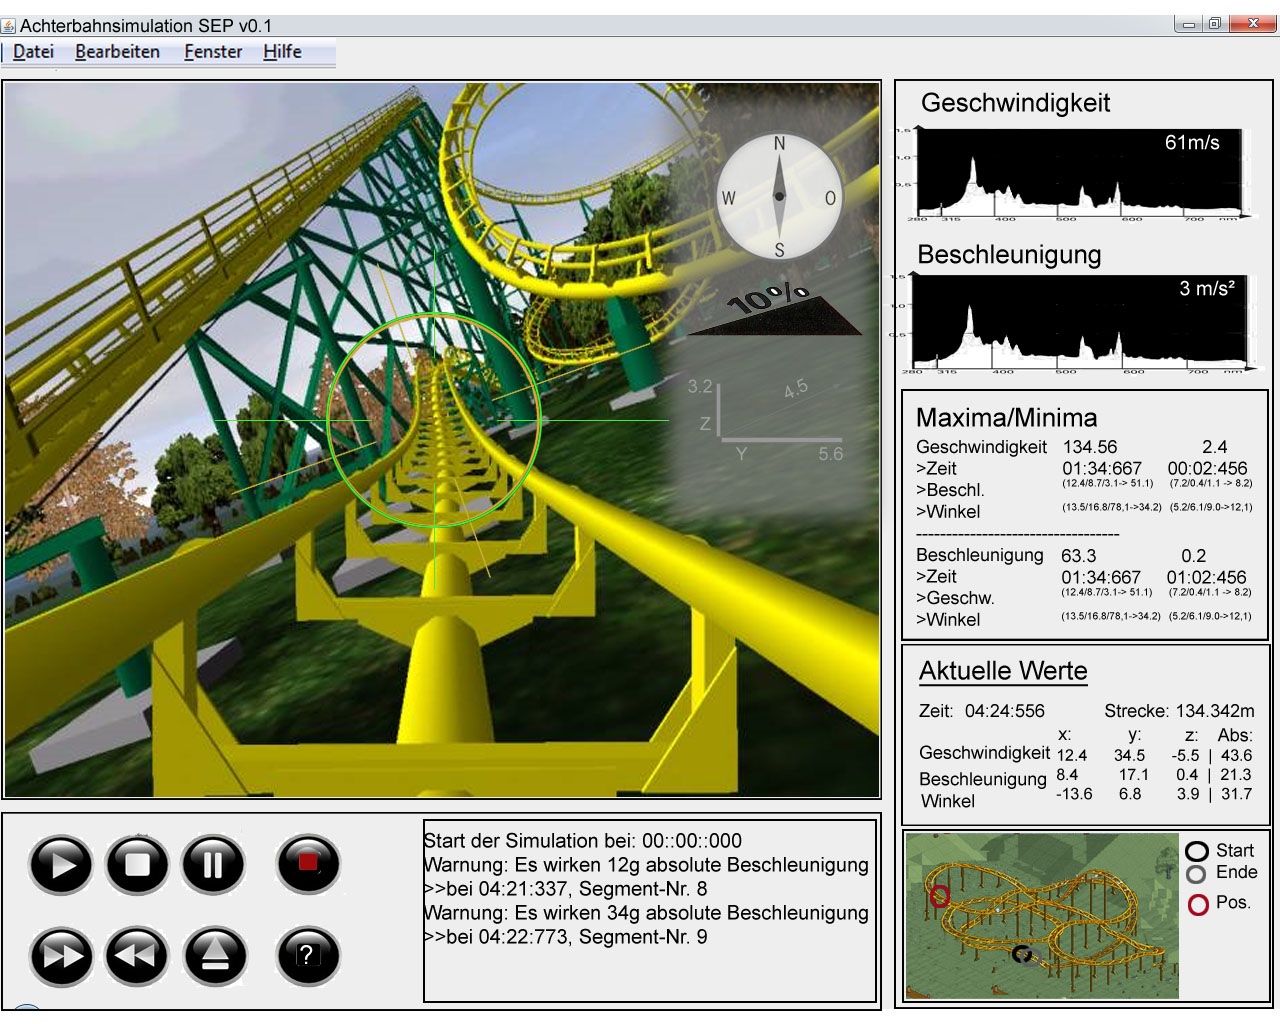
\includegraphics[width=0.75\linewidth]{GUI_v2.jpg}
			\caption{W"ahrend der Simulation}
		\end{figure}
	\end{frame}
	
	\section{Komponenten}
	\begin{frame}{Komponenten}
		\begin{figure}
			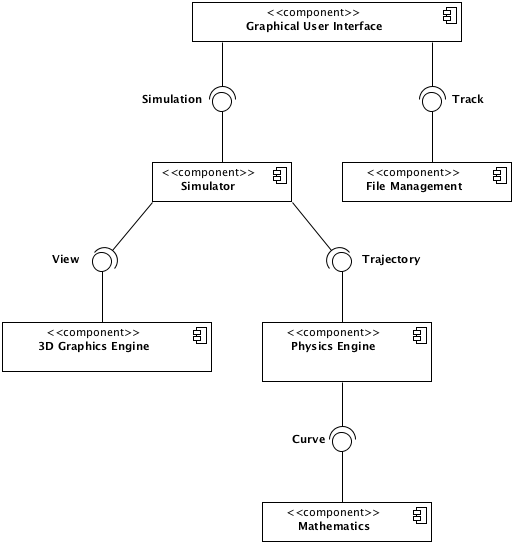
\includegraphics[width=0.55\linewidth]{component_overview.png}
			\caption{Komponentendiagramm}
		\end{figure}
	\end{frame}
	
	
\end{document}
